


\chapter{Přehled použitých metod}

V této kapitole jsou popsány konkrétní metody detekce, popisu a asociace obrazových příznaků.

\section{Moravec}

Jedná se o nejstarší a nejjednodušší uvedený operátor pro nalezení bodových příznaků \cite{moravec1980obstacle}. Je uveden proto, že představuje primitivní ideový základ pro další uvedené operátory. Jeho principem je představa že, hledaný příznakový bod by měl vynikat ve všech směrech kolem sebe, tj. že by na všechny strany od něj měla být výrazná změna v jasu. Algoritmus Moravec je pouze detektor, deskriptor ani doporučení stran porovnávání bodů nejsou jeho součástí.

\subsection{Algoritmus}

Průměrná změna jasu v okolí bodu ve směru posunu (x,y) je definována jako:
\begin{align}	
E_{x,y} = \sum_{u,v} w_{u,v} \lvert I_{u+x, v+y} - I_{u,v} \rvert^2 , (x,y) \in \{(1,0), (1,1), (0,1), (-1,1)\},
\end{align}

\begin{figure}[htp] 
	\centering{
		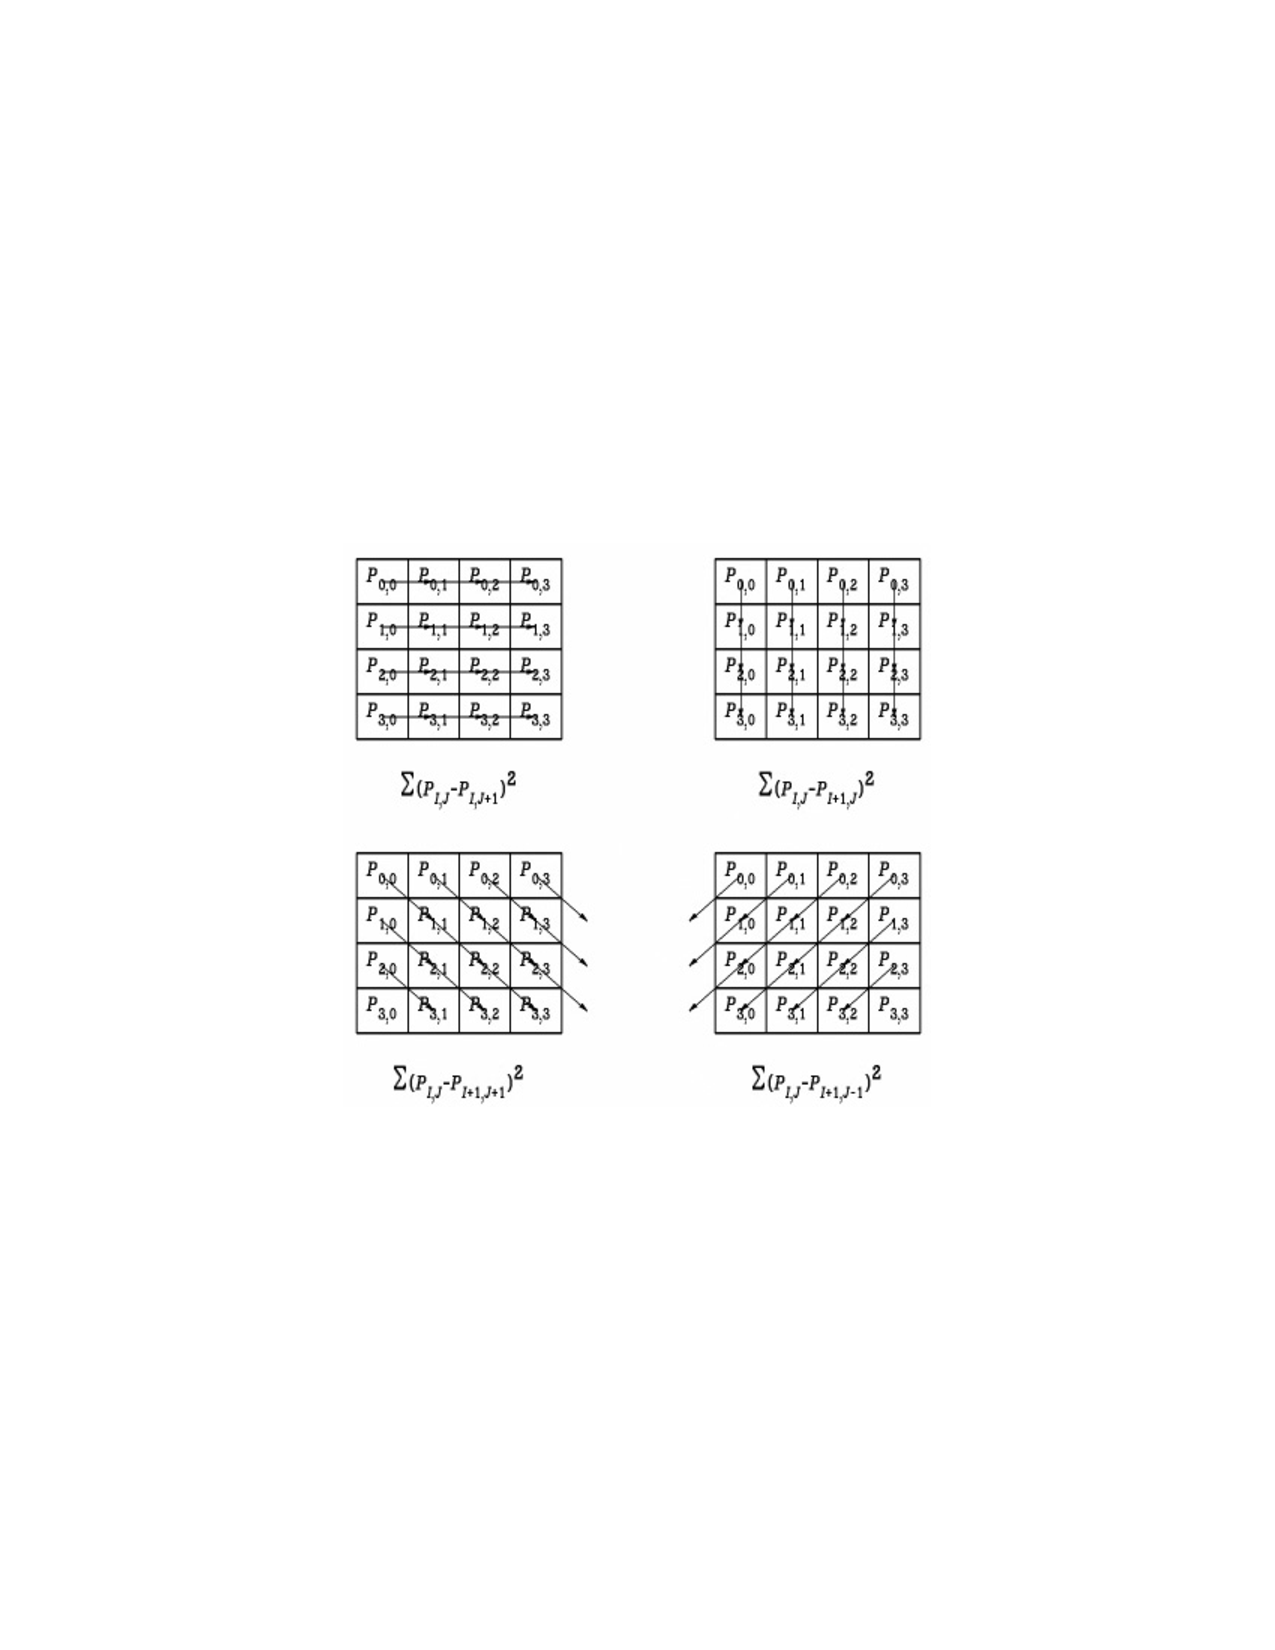
\includegraphics[scale=0.7]{text_img/moravec_posun.pdf}}
	\caption{Vizualizace posunů v jenodlivých směrech} 	\label{Moravec_posun}
\end{figure}
	
kde  $I$ je obraz ve formě jasových bodů, $w$ je váhové okénko (algoritmus používá čtvercové binární), $(u,v)$ je aktuální pozice v obrazu a $(x,y)$ je aktuální posun. Provede se tedy posun všech obrazových bodů danými směry, a  původní varianta se vždy odečte od posunuté. Tím je získána informace o změně jasu při posunutí ve směrech  $\alpha \in \{0, 45, 90, 135\}$ stupňů. Poté je každé testované místo (každý pixel) překryto čtvercovým okénkem, hodnoty pod ním sečteny a výsledek umocněn na druhou. Pro každé testované místo tedy vzniknout 4 hodnoty čtverce změny v jednotlivých směrech.
Ve zbytku algoritmu je pro každé místo vybráno $min\{E_{x,y}\}$, v takto vzniklém obrazu se stanoví určitý práh a body s vyšší hodnotou, než je tento práh jsou označeny jako výsledné příznaky.

Jedná se tedy o nalezení bodů, které mají diskrétní diferenci v daných směrech nejméně takovou, jaká je odmocnina
hodnoty prahu.

\subsection{Využití}
Tento operátor má řadu nedostatků, zejména:
\begin{itemize}
	\item Je anizotropní: uvažuje pouze změny v diskrétních úhlech, které jsou násobky 45 stupňů. Změnám v ostatních úhlech bude logicky přiřazen nižší význam
	\item Binární čtevrcové okénko výsledek výpočtu zašumuje
	\item Příliš citlivý: protože reaguje pouze na nejmenší změnu intenzity.
\end{itemize}

Dnes se již prakticky nevyužívá, ale stal se základem dalších algoritmů.

\section{Harris}
		
Algoritmus Harris \cite{harris1988combined} vznikl snahou odstranit nedostatky operátoru Moravec - pracuje se stejnou představou, ale efektivněji.

\subsection{Algoritmus}	
\label{harris_alg}

Anizotropní vlastnosti lze odstranit pomocí Taylorova rozvoje:
\begin{align}	
E_{x,y} = \sum_{u,v} w_{u,v} \lvert I_{x+u, y+v} - I_{u,v} \rvert^2
\approx \sum_{u,v} w_{u,v} \lvert I_{u, v} + xX + yY  - I_{u,v} \rvert^2
\end{align}
\begin{align}
E_{x,y} = \sum_{u,v} w_{u,v} \lvert xX + yY \rvert^2
\end{align}

kde $(x,y)$ je vektor podle kterého se derivuje a $X$ a $Y$ jsou aproximované parciální derivace obrazu ve směrech osy x a osy y:
\begin{align}
X = I \otimes (-1, 0, 1) \approx \frac{\delta I}{\delta x}
\end{align}
\begin{align}
Y = I \otimes (-1, 0, 1)^T \approx \frac{\delta I}{\delta y}
\end{align}
\begin{align}
E_{x,y} = \sum_{u,v} w_{u,v} [x^2X^2 + 2xyXY + y^2Y^2]
\end{align}
označme:
\begin{align}
M = \sum_{u,v} w_{u,v} 
\begin{bmatrix}
X^2  \  XY \\
XY    \ Y^2 \\
\end{bmatrix}
\end{align}
výsledný vztah:
\begin{align}
E_{x,y} = [x, y] M \begin{bmatrix} x \\ y \end{bmatrix}
\end{align}
Tento vztah vyjadřuje velikost gradientu obrazu ve směru (libovolného) vektoru $(x,y)$. Matice $M$ je někdy nazývána Harrisova matice.
Pokud je místo čtvercového okna nyní zvoleno gaussovské:
\begin{align}
w_{u,v} = e^{-(u^2 + v^2)/2\sigma^2},
\end{align}
je odstraněn první problém operátoru Moravec: zanášení šumu do výpočtu nevhodným ("ostrým") okénkem. Směr a velikost derivací je nyní popsán elipsou ve formě matice M, která respektuje celý kruhový prostor kolem bodu a velikost os této elipsy není závislá na rotaci obrazu. 

Velikosti os této elipsy jsou popsány velikostí vlastních čísel matice, tj. pro:

\begin{itemize}
	\item ${\lambda_1 \approx 0 \wedge \lambda_2 \approx 0}$ - se v tomto bodě příznak nenachází, pro
	\item ${\lambda_1 \approx 0 \wedge \lambda_2 \gg 0}$ nebo naopak - tímto bodem prochází hrana a pro
	\item ${\lambda_1 \gg 0 \wedge \lambda_2 \gg 0}$  - se v tomto bodě nachází roh.
\end{itemize}

%\includepdf{[scale=0.3]Harris_eigen.pdf}

Protože výpočet vlastních čísel matice je relativně náročná operace, zatímco determinant a stopu matice $2\times2$ lze získat prostým odčítáním a násobením, původně Harris navrhuje tento výpočet aproximovat jako:

\begin{align}
R = \text{det}(M) - k * \text{stopa}(M)^2,
\end{align}
kde det$(M)$ je determinant matice $M$, stopa$(M)$ je součet prvků na hlavní diagonále čtvercové matice a $k$ je nastavitelná konstanta, která určuje citlivost algoritmu na hrany. $R$ bude nabývat hodnot:
\begin{itemize}
	\item malých pro "plochou"\ oblast bez velkých změn
	\item kladných pro roh nebo jiný bodový orientační bod
	\item záporných pro hranu
\end{itemize} 

Body se tedy označí porovnáním $R$ se zvoleným prahem.

\begin{figure}[htp] 
	\label{Harris_eigen}
	\centering{
		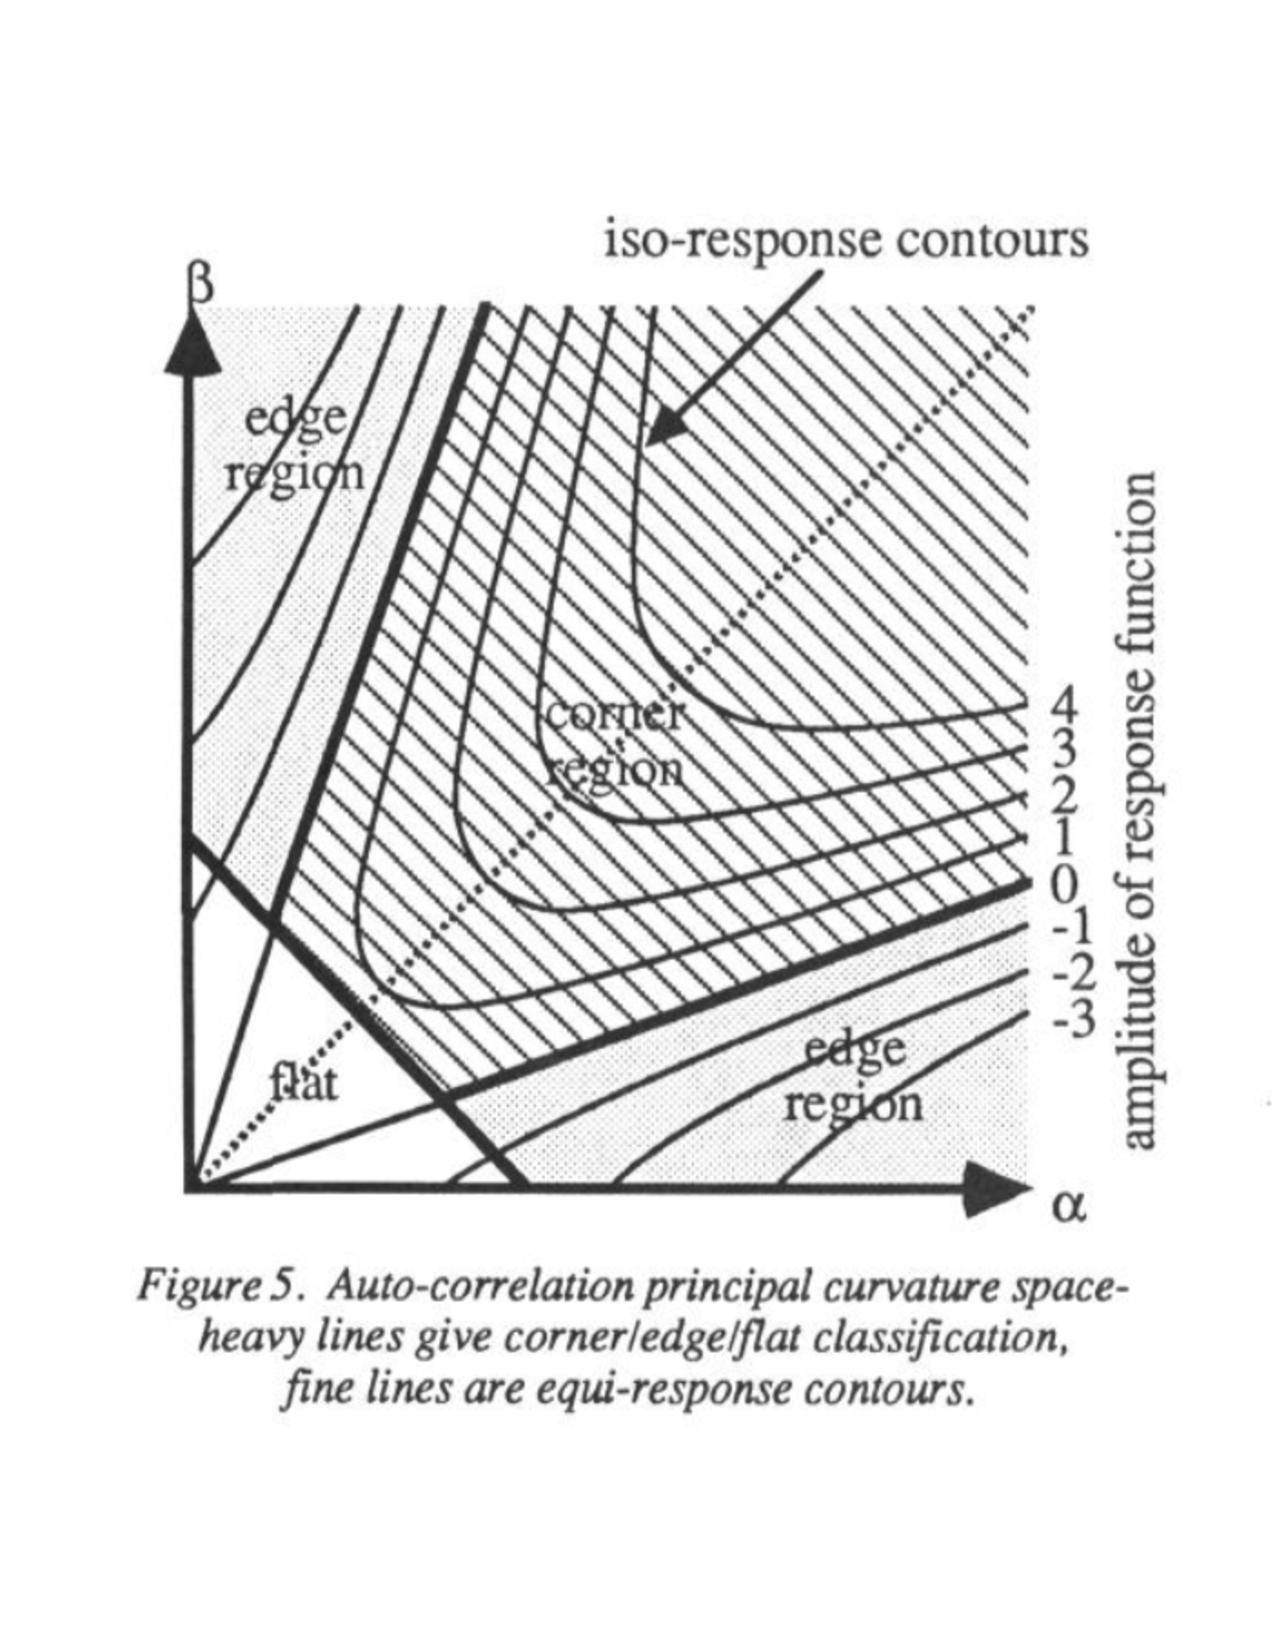
\includegraphics[scale=0.3]{Harris_eigen.pdf}}
	\caption{Vliv tvaru okolí bodu na rozložení vlastních čísel matice M}
\end{figure}


\subsection{Využití}
V algoritmu Harris jsou odstraněny hlavní nedostatky algoritmu Moravec. Zašumování výsledků nahrazením čtvercového okna gaussovským a anizotropické vlastnosti a přílišnou citlivost na nejnižší derivaci reprezentací derivací v bodě jako 2D elipsy jejíž osy jsou určeny vlastními čísly matice M (a aproximovány výše uvedeným vztahem pro $R$). Jeho velkou výhodou oproti dalším metodám je nenáročnost na výkon hardwaru.

\section{Shi-Tomasi}

	Protože detekování hran jako příznakových bodů není z hlediska jejich sledování vhodné (body na hranách jsou logicky nejednoznačné a navzájem velmi podobné), navrhli Shi a Tomasi \cite{shi1994good} vylepšení Harrisova algoritmu tak, aby detekoval pouze rohy. Toho lze dosáhnout pomocí výpočtu $R$ přímo z vlastních čísel (vysvětlení viz \ref{harris_alg}). 
	
	\begin{align}
	R = min(\lambda_1, \lambda_2)
	\end{align}
	
	Body se opět označí porovnáním $R$ se zvoleným prahem. Výhodou tohoto řešení je zlepšení vlastností příznaků pro sledování za cenu mírného zvýšení výkonové náročnosti. Tento algoritmus bývá také nazýván Good Features to Track, zkráceně GFTT, podle názvu článku ve kterém byl původně popsán.

\section{FAST}

	Jak název algoritmu napovídá, jedná se o rychlou a jednoduchou metodu nalezení bodových příznaků v obraze. Autoři uvádějí dvakrát větší rychlost, než vykazuje SIFT (sekce \ref{sec:sift}) a dokonce větší, než Harris. Obě tato tvrzení byla potvrzena v kapitole \ref{chap:impl}. Jedná se o čistou detekci příznaků, algoritmus neobsahuje deskriptor nebo metodu porovnávání příznaků. Z FAST \cite{rosten2010faster} ale vychází detektor systému ORB popsaný v sekci \ref{sec:orb}.
	
	\begin{figure}[htp] 
		\centering{
			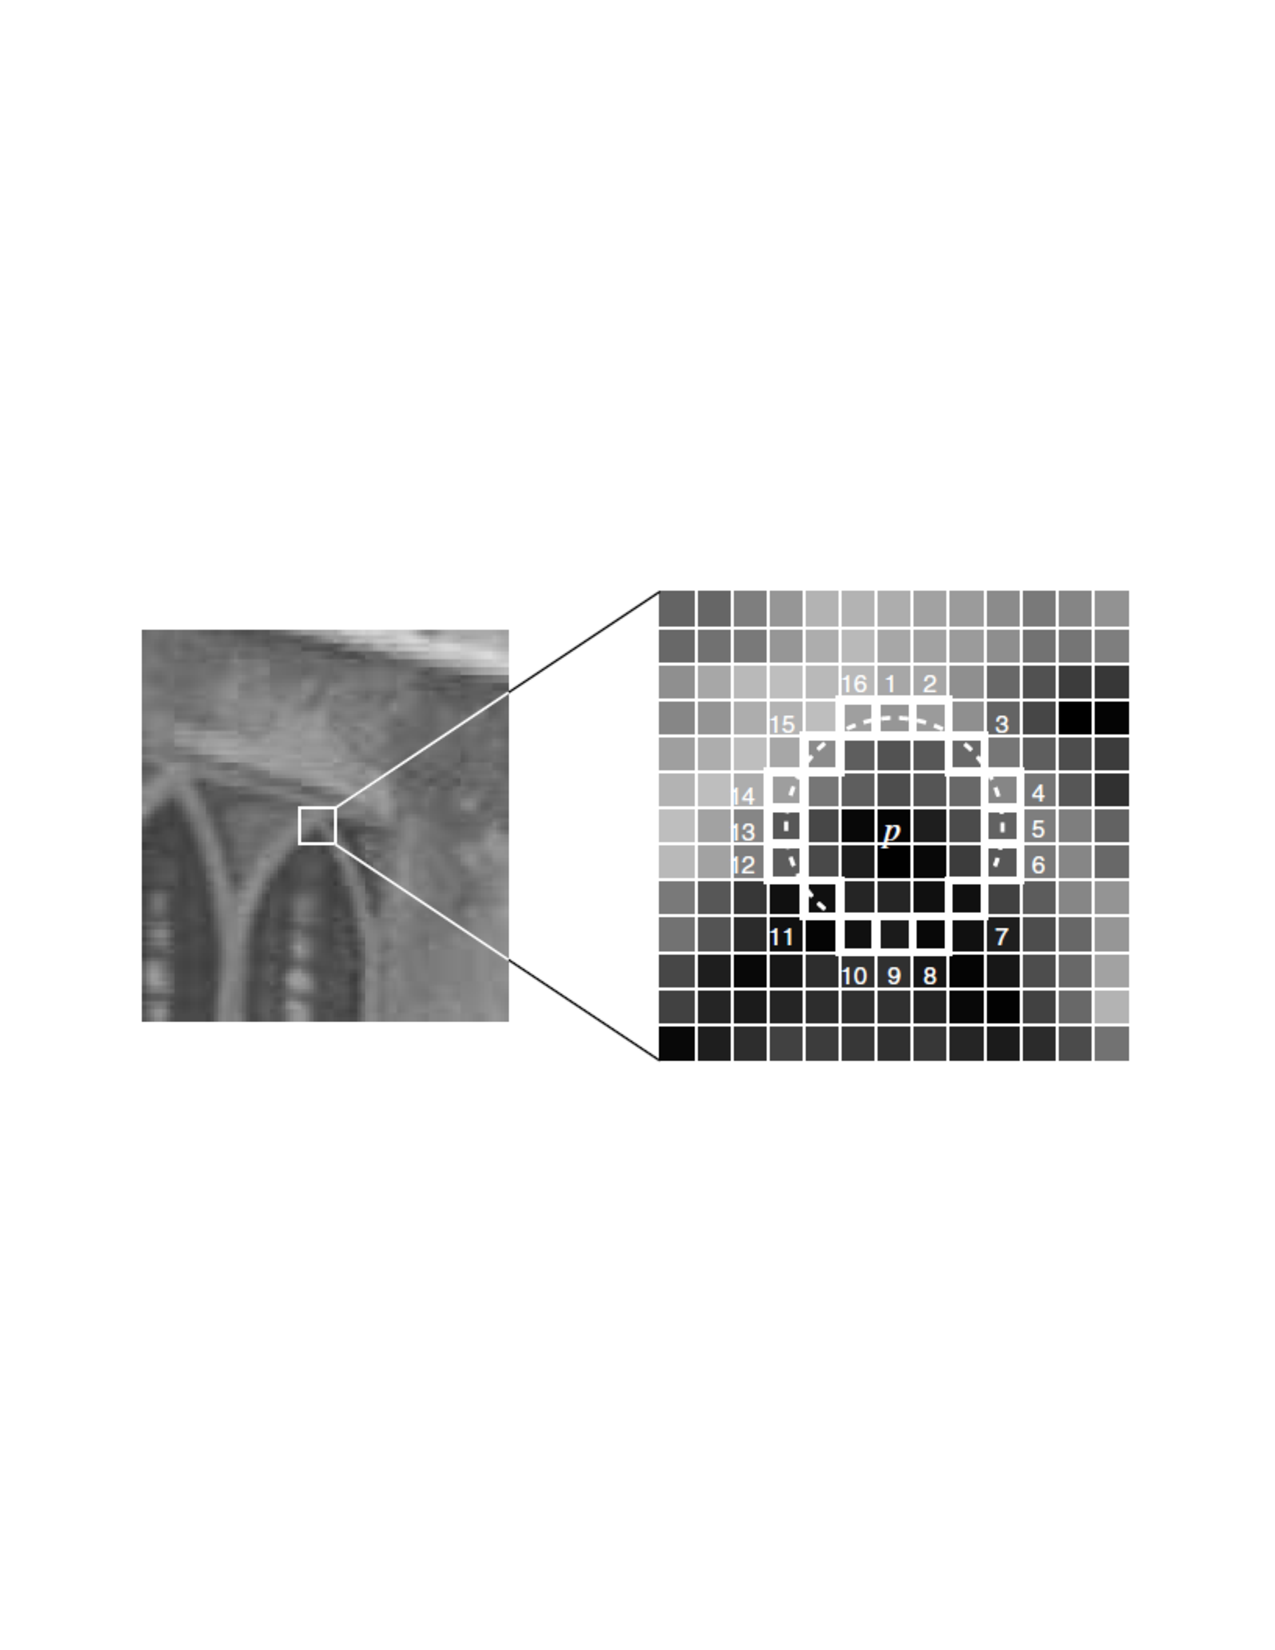
\includegraphics[scale=0.7]{text_img/fast_corner.pdf}}
		\caption{Extrakce FAST příznaku} 	\label{fast_corner}
	\end{figure}
	
	\subsection{Algoritmus}
	
		\begin{enumerate}
			\item Okolo testovaného bodu $t$ se zkonstruuje kružnice sestávající z 16 bodů $t_{1-16}$. 
			\item Je-li v kružnici $n$ (doporučuje se $n=12$) nebo více spojených bodů takových, že $\lvert I(p) - I(t_i) \rvert > T$, bod je označen za příznak. $I(.)$ je intenzita daného bodu, $T$ je definovaný práh rozdílu intenzit.
			\item Protože algoritmus má tendenci označit jako příznaky mnoho sousedících bodů, je vhodné po nalezení všech příznaků provést potlačení nemaximálních hodnot (ang. Non-maximum supression). To zajistí, že se z každé spojené oblasti sousedících příznakových bodů vybere jen ten, který má největší nebo nejmenší intenzitu a ostatní se zahodí.
		\end{enumerate}
		
		Autoři dále navrhují vylepšení popsaného algoritmu testováním nejprve 2 nebo 4 pixelů v bodu 2 a pokračování pouze pokud tyto body splňují definovanou podmínku. Otázka, které body na pro tento test zvolit, je řešena nasazením neuronové sítě, která se na určitých datech natrénuje tak, aby tento test byl pro detekci příznaků co nejinformativnější.
		
	\subsection{Využití}
	
		FAST příznaky našly využití například ve SLAM systému PTAM (parallel tracking and mapping) a často jsou nasazovány v aplikacích na mobilních telefonech, jejichž výkon je oproti desktopům stále limitován.	
	 

\section{SIFT}
\label{sec:sift}
	SIFT \cite{lowe2004distinctive} je metoda vyhledání příznakových bodů v obraze spolu s výrobou deskriptorů pro jejich zpětnou identifikaci při dalším nalezení. Navazuje na předchozí algoritmy typu Harris, její výhodou je však větší robustnost vzhledem k zašumění obrazu, změnám osvětlení, afinním transformacím příznakových bodů a jejich pohybu v prostoru. Deskriptory se vyznačují velkou rozpoznatelností, tzn. různé body nebudou mít podobný deskriptor.
	
	Lze ji využít nejen k identifikaci bodů pro prostorovou lokalizaci, ale též k robustnímu hledání definovaných objektů v obrazu, kdy objekty jsou reprezentovány množinou charakteristických bodů.
	
	Algoritmus extrakce deskriptorů je uspořádán do kaskádovité struktury  za účelem urychlení výpočtu: Složitější operace jsou umístěny co  nejdále v algoritmu tak, aby byly aplikovány až po filtraci, tj na co nejmenší množství dat.
	
	\begin{figure}[htp] 
		\centering{
			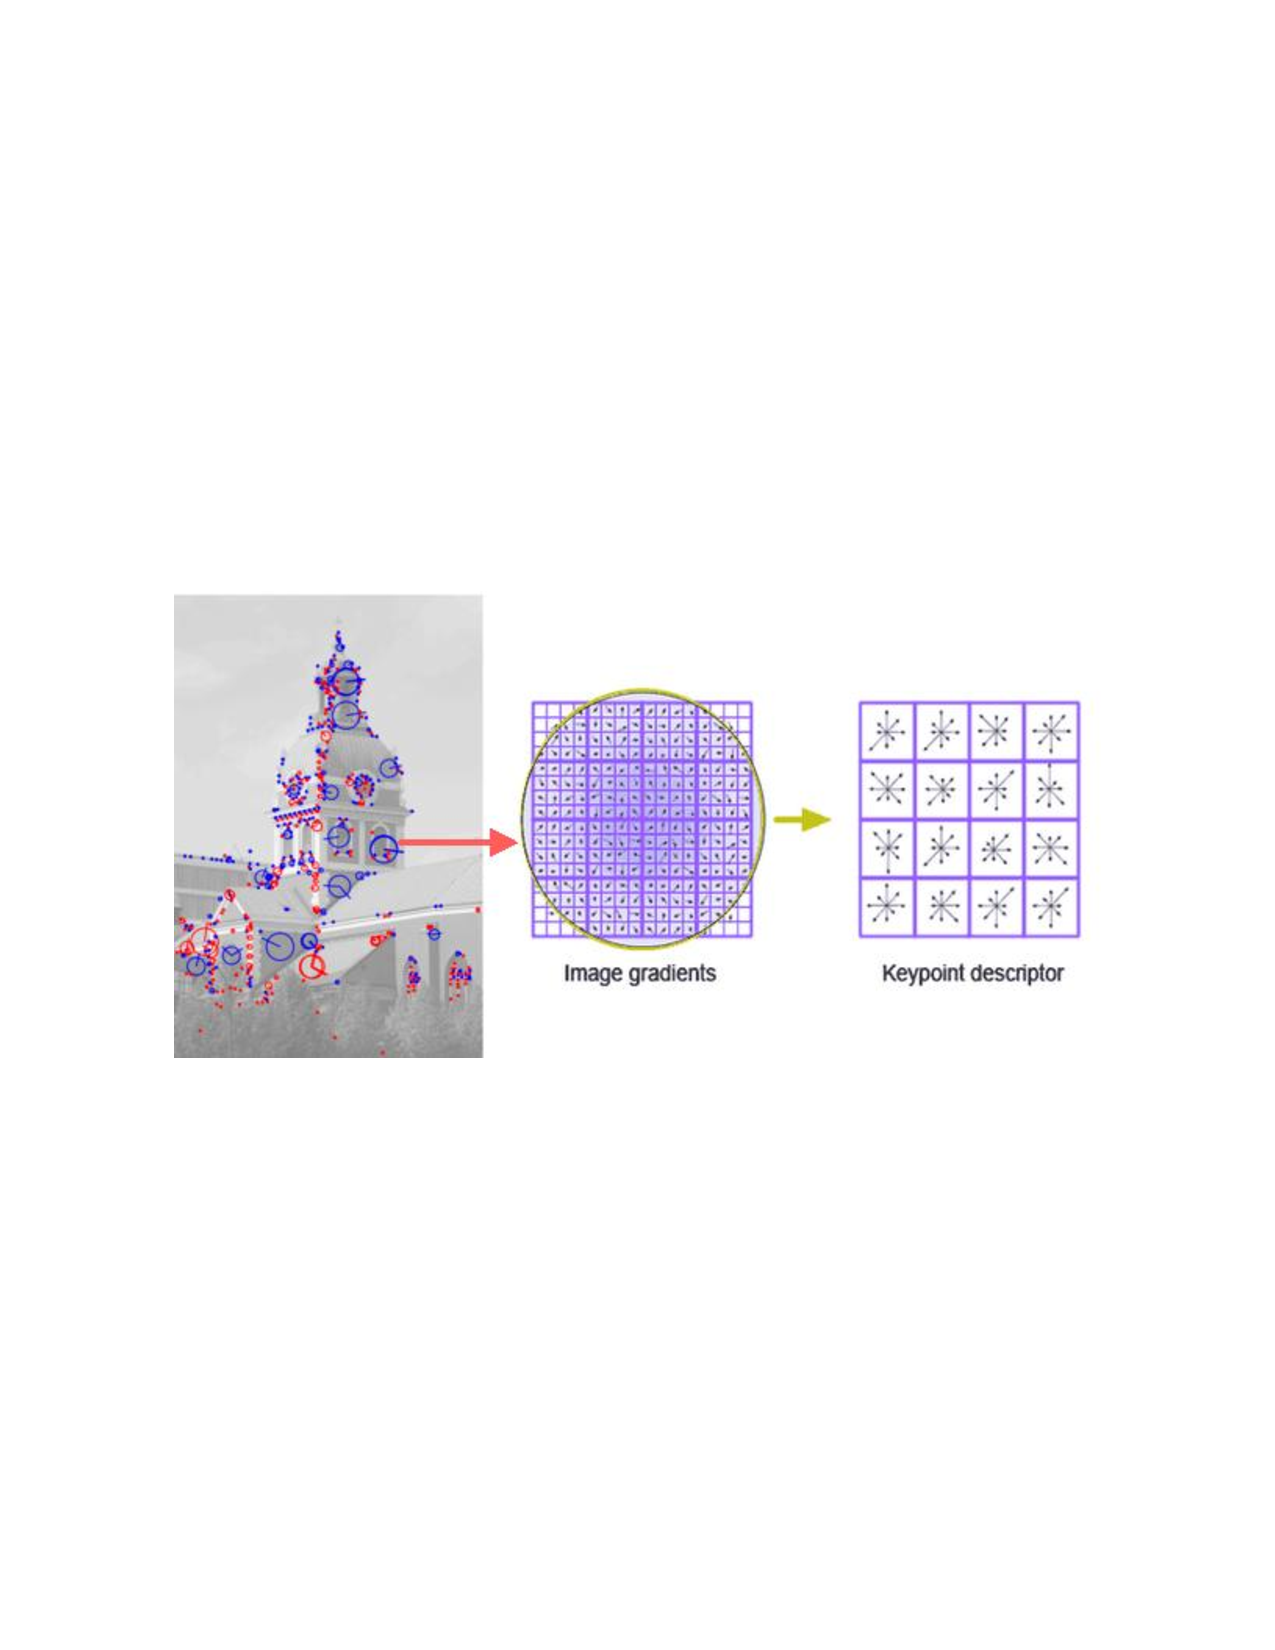
\includegraphics[scale=0.8]{text_img/sift_kp.pdf}}
		\caption{Extrakce SIFT deskriptoru} 	\label{sift_kp}
	\end{figure}
	
	\subsection{Algoritmus detekce příznaků}
	
	\begin{enumerate}
		\item Hledání jasových extrémů v celém obrazu nezávisle na zvětšení, neboli měřítku: Provede se pomocí rozdílů gaussianů (Difference-of-Gaussians, DoG).
			
			Pracuje se s matematickou konstrukcí laplaciánu gaussiánů, což znamená rozdělení obrazu na pyramidu postupně více rozostřených verzí (rozostření se provede pomocí gaussovského jádra - masky se vzrůstajícím rozptylem $\sigma{}$). Laplacián poskytne spojitou alternativu rozdílů mezi jednotlivými úrovněmi tohoto postupného rozostření. Tento postup zajišťuje, že najdeme-li někde v těchto "rozdílech"\ příznakový bod, nalezneme ho stejně i v jiném obrazu, kde se bude nacházet v jiném měřítku. V takovém obraze se bude příznak nacházet jinde v tomto prostoru rozostření, ale bude vypadat stejně, což umožňuje porovnání nezávisle na měřítku.
			
			Protože výše popsaný postup platí pro spojitý prostor, při práci s diskrétním obrazem se aproximuje vytvořením pyramidy postupně více a více rozostřených vrstev, kdy tuto pyramidu ještě rozdělíme do oktáv (anglicky octaves). Nejvyšší rozostření oktávy v SIFTu by mělo mít oproti nejnižšímu dvojnásobný rozptyl $\sigma$. Jedná se o analogii hudebního názvosloví, kdy nejvyšší tón oktávy má oproti nejnižšímu dvojnásobnou frekvenci v hertzích. V další oktávě se též oproti předchozí pracuje s dvojnásobně redukovaným rozlišením obrazu (každý druhý řádek, každý druhý sloupec), protože se předpokládá, že dojde jenom k malé ztrátě informace při značném snížení výkonových nároků.
			
			Tuto pyramidu gaussiánů doporučují autoři článku \cite{lowe2004distinctive} konstruovat tak, že se skládá ze 4 oktáv po 5 rozostřeních (měřítkách, ang. scales), první rozostření se doporučuje $\sigma_0 = 1.6$ a rozdíly jednotlivých rozostření jsou $k=\sqrt{2}: \sigma_2 = k \sigma_1 = k^2 \sigma_0$ atd. Podstatné je dodržet konstantní $k$ mezi vrstvami.
			
			Z této pyramidy gaussiánů se vytvoří pyramida jejich rozdílů prostým odečtením následujících vrstev v pyramidě a vznikne v úvodu zmíněný DoG operátor.		
			
		\begin{figure}[htp] 
			\centering{
				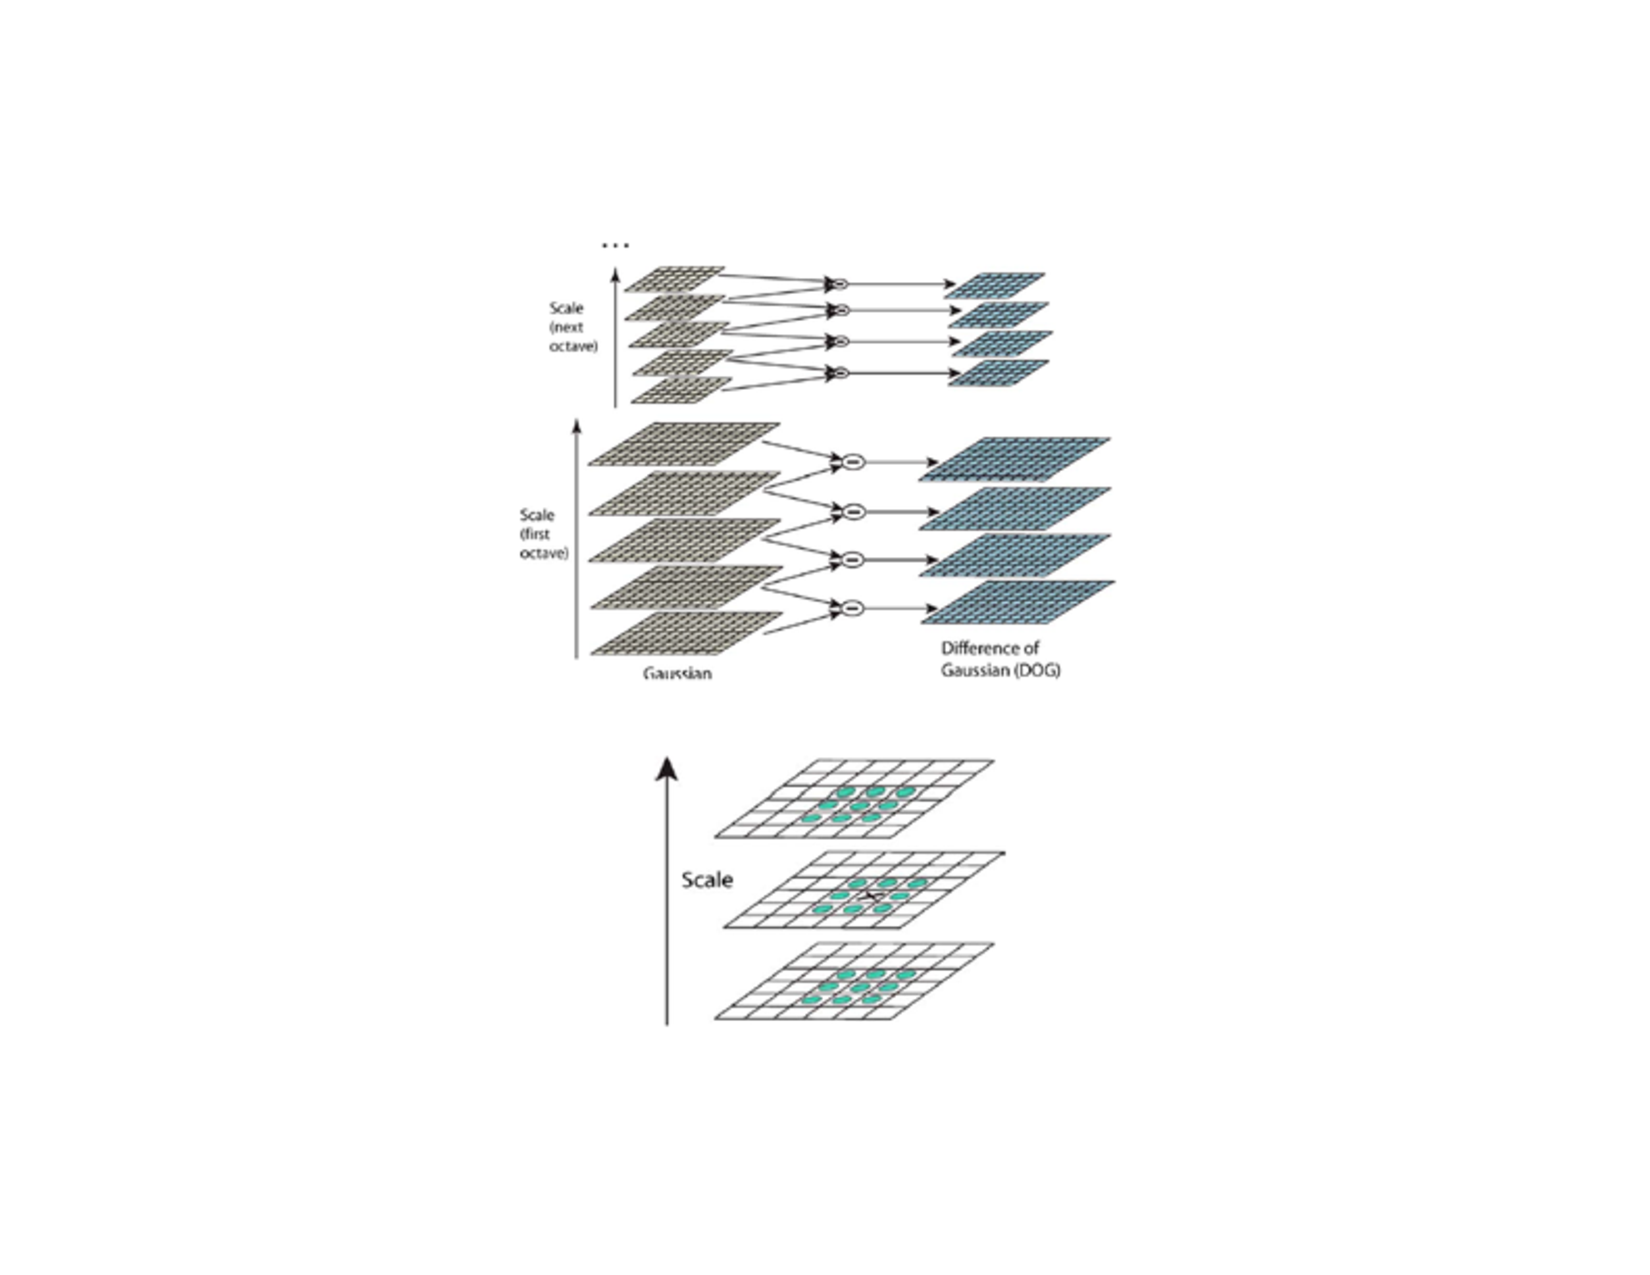
\includegraphics[scale=0.6]{text_img/sift_dog.pdf}}
			\caption{Tvorba DoG pyramidy} 	\label{sift_dog}
		\end{figure} 
			
		\item Lokalizace klíčových oblastí: Na každé kandidátské lokaci se provede rozhodnutí o umístění a relativní velikosti oblasti. Klíčové oblasti jsou vybrány na základě měřítek jejich stability
		
			Každý bod výsledné pyramidy z předchozího kroku se porovná s celkem 26 svými sousedy: 8 bezprostředně příléhajícími ve své vrstvě a oknem 3x3, tedy 9 bodů na stejné lokaci ve vrstvě nad a pod. Za kandidáta se bod označí v případě, že má ze všech těchto sousedů největší nebo nejmenší intenzitu. (v krajních vrstvách oktáv se nehledá, neboť jim chybí sousední vrstva nad nebo pod).
			
			Kolem takového kandidátského bodu lze za účelem dosažení subpixelové přesnosti zkonstruovat trojrozměrnou plochu pomocí Taylorova rozvoje:
			
			\begin{equation}
			\label{rozvoj}
			D(\mathbf{x}) = D(\mathbf{x_0}) + \frac{\delta D(\mathbf{x_0})}{\delta \mathbf{x}} \mathbf{x} + \frac{1}{2} \mathbf{x^T}\frac{\delta{}^2 D(\mathbf{x_0})}{\delta{}\mathbf{x^2}}\mathbf{x}, 
			\end{equation}
			
			\begin{equation} \mathbf{x} = [x, y, \sigma{}], \end{equation}
	
			a za skutečné umístění příznaku označit její extrém, tedy bod, kde je derivace této funkce nulová:
			
			\begin{align}
			\mathbf{\hat{x}} = - \frac{\delta{}^2 D(\mathbf{x_0})^{-1}}{\delta{}\mathbf{x^2}}
			\frac{\delta D(\mathbf{x_0})}{\delta \mathbf{x}},
			\end{align}
			
			Pro další zpřesnění lze do rovnice \ref{rozvoj} dosadit vypočtený bod $\hat{\mathbf{x}}$. Pokud má funkce v tomto bodě v kterémkoli směru větší hodnotu než 0.5, znamená to, že by se jako střed příznaku měl zvolit spíše bod, který se nachází tímto směrem.
			
			Poslední operací tohoto kroku je vyřazení bodů, které se nacházejí na hranách, neboť ty nelze považovat za spolehlivé příznaky. Pomocí Hessovy matice \ref{hess_matr} se vypočte zakřivení plochy \ref{rozvoj} v okolí bodu a to se porovná s níže prahovým výrazem. Jde o podobný princip jako je eliminace hran v algoritmech Harris nebo Shi-Tomasi.
			
			\begin{align}
			\label{hess_matr}
			H = \begin{bmatrix}
			D_{xx} && D{xy} \\
			D_{xy} && D{yy}
			\end{bmatrix},\\
			\frac{Tr(H)^2}{Det(H)} < \frac{(r+1))}{r},
			\end{align}
			$r$ je volitelná prahová konstanta. Její hodnotu  autoři \cite{lowe2004distinctive} doporučují 10.
			
								
		\item Určení orientace: Ke každé klíčové oblasti je přiřazena jedna nebo více orientací podle směrů lokálních gradientů. Další operace se provádějí na oblasti, která je transformovaná pomocí informací o relativní velikosti, umístění a orientaci aby bylo dosaženo nezávislosti deskriptoru a na těchto  vlastnostech
		
			Pomocí lokálních diferencí se určí velikost a směr gradientů zvoleného počtu bodů okolo nalezeného příznaku podle os $x$ a $y$. Tyto gradienty se kvantizují do 36 kategorií po 10 stupních. Pak se stanoví maximum tohoto histogramu a pokud druhá nejvyšší hodnota histogramu dosahuje alespoň 80\% hodnoty té nejvyšší, stanoví se pro tento příznak dvě orientace. Přesné úhly orientací se nakonec stanoví pomocí proložení kvadratické křivky maximem histogramu a jeho dvěma sousedy a maximalizací této křivky.	
					
		\item Výroba deskriptoru oblasti: Na každé dané oblasti jsou vypočteny lokální gradienty. Ty jsou převedeny do tvaru invariantního k deformaci tvaru a změnám osvětlení.
		
			V tomto bodě se vypočtou gradienty čtvercového okolí 16x16 pixelů okolo zvoleného bodu. Jejich velikosti se přenásobí gaussovým oknem pro zvýraznění těch, které jsou blízko středu. Tato oblast se poté rozdělí na 16 oblastí se 4x4 pixely. V každé této oblasti se vypočte histogram gradientů a nakvantizuje se do 8 kategorií podobně jako v předchozím kroku.
			
			Výsledkem je SIFT deskriptor: 16 histogramů gradientů po 8 orientačních kategoriích (binech), tedy matice 4x4x8. Jako poslední krok se tento vektor normalizuje na jednotkovou délku aby se potlačily vlivy osvětlení. 
			
			
	\end{enumerate}
	
	Algoritmus vytváří velké množství příznaků, které hustě pokrývají celou plochu obrazu (cca 2000 příznaků na obraz 500x500px). Tyto příznaky je potřeba uchovávat v databázi a implementovat algoritmus pro její správu.
	
	Výsledný deskriptor je trojrozměrná matice 4x4x8, příznaky se porovnávají pomocí algoritmu nalezení nejbližšího souseda, resp. jeho aproximace.
	
	\subsection{Porovnávání příznaků}
	
	Pro porovnávání příznaků autoři doporučují algoritmus nejbližšího souseda a pro větší databáze jeho aproximaci Best Bin First (sekce \ref{sec:bbf}). Tento algoritmus dělí prostor příznaků na diskrétní disjunktní oblasti, odhaduje, ve kterém se hledaný prvek pravděpodobně nachází a hledá ho nejprve tam. Autoři uvádějí, že oproti standartnímu nejbližšímu sousedovi tento algoritmus zrychluje výpočet o dva řády za cenu pouze 5\% ztráty přesnosti.
	
	\subsection{Využití}
	
	SIFT je stále jedním z nejspolehlivějších algoritmů hledání a identifikace příznaků, což dokazuje i jeho široká využívanost v aplikacích identifikace objektů podle známých příznaků i v mapovacích algoritmech (Monoslam, \cite{slam_monoslam} ). Ikdyž ho lze využít pro mapování v reálném čase, je v porovnání s ostatními metodami velmi výkonově náročný. Jeho převaha nad ostatními uvedenými metodami s výjimkou SURF se zřetelně projevila při testech v kapitole \ref{chap:impl}


\section{SURF}

	Speeded up robust features neboli SURF \cite{bay2006surf} je metoda, která ideově navazuje na SIFT - jedná se o jeho aproximaci. Namísto konstrukce aproximace laplaciánu postupným rozostřováním jako v u SIFTu se předpokládá, že výskyt příznaků závisí čístě na determinantech Hessovských matic, jejíž hodnota se velmi rychle odhadne pomocí filtrací obdélníkovými filtry.
	
	Při výrobě deskriptoru se namísto gradientů z lokálních diferencí použijí Haarovské waveletové filtry, z jejichž aplikací se odhadne orientace i přímo sestaví deskriptor. 
	
\subsection{Algoritmus}

	\begin{enumerate}
		\item Nejprve je zkonstruována aproximace laplaciánu - konvolucí daných diferenčních filtrů s postupně rostoucí velikostí, kdy jeden filtr reprezentuje $D_{xx}$, druhý $D_{xy}$ a poslední $D_{yy}$ je aproximována Hessova matice:
		\begin{align}
			H = \begin{bmatrix}
			D_{xx} && D_{xy} \\ 
			D_{xy} && D_{yy}
			\end{bmatrix}
		\end{align}
		Prvky jedné úrovně pyramidy se skládají z aproximace determinantu této matice: $det(H) = D_{xx}D_{yy} - (0.9D_{xy})^2$. Jednotlivé úrovně se potom liší velikostí filtru viz výše: začíná se na velikosti 9x9, která odpovídá $\sigma = 1.2$ v SIFTu. S každou vrstvou se k velikosti filtru přičítá fixní konstanta, začíná se na 6, což reprezentuje zdvojnásobení parametru $\sigma$ u SIFTu. Pyramida se opět dělí do oktáv. Změna velikosti filtru se mezi oktávami zdvojnásobuje.
			
		\item Za příznak se opět označí extrém v tomto prostoru. Stejně jako u SIFTu je použito potlačení nemaximálních hodnot(non-maximum supression). Bod se porovná se svým okolím 3x3x3 v rámci pyramidy a za příznak je vzat v momentě, kdy je z něj nevětší nebo nejmenší.
		
		\item Deskriptor je z okolí bodu syntetizován následujícím způsobem: Nejprve se vypočte reakce na Haarovy waveletové obdelníkové filtry ve směrech $x$ a $y$. Označíme $d_x, d_y$. Výpočet probíhá na kruhovém okolí bodu s poloměrem $16\sigma$, filtry mají velikost $4\sigma$. 
		
		Výsledek ($d_x, d_y$) je převážen gaussovskou maskou se středem v bodě příznaku a rozptylem $\sigma_{G} = 2.5\sigma{}$. Výsledný prostor je rozdělen na 16 úhlových výsečí po 60 stupních. Hodnoty v jednotlivých výsečích se sečtou a maximum těchto součtů určuje dominantní směr.
		
		Okolo bodu příznaku se extrahuje okno $20\sigma{} \times 20\sigma{}$. Toto okno se otočí o vypočtený dominantní úhel za účelem dosažení invariance k rotaci příznaku. Opět se vypočtou reakce na Haarovy waveletové filtry ve směrech x a y, ty se znovu převáží Gaussovskou maskou, tentokrát s rozptylem $\sigma_G = 3.3\sigma$. 
		
		Toto okolí se rozdělí na výseče 4x4 body a pro každou se vypočte 
		
		\begin{align}
		v = [\sum d_x, \sum d_y, \sum\lvert d_x \rvert, \sum\lvert d_y \rvert ],
		\end{align}
		
		což je finální dekskriptor.
		
	\end{enumerate}
	
	\subsection{Využití}
		
		Přestože je SURF původně navržen jako rychlá aproximace SIFT, v hodnocení detektorů v kapitole \ref{chap:impl} měl vyšší průměrný čas detekce než SIFT, zato ale vykazoval čtyřikrát kratší celkový čas deskripce a dokonce překonal SIFT v celkovém hodnocení zejmena díky lepším výsledkům na datasetech s rotací. 

\section{BRIEF}
\label{sec:brief}
	Binary Robust Independent Elementary Features neboli BRIEF \cite{calonder2010brief} je deskriptorový algoritmus, zabývá se tedy pouze popisem příznaků, nikoli jejic nalezením. Jeho principem je popis příznaků pomocí řetězce binárních hodnot. To je výhodné, protože takové řetězce lze porovnávat pomocí Hammingovy vzdálenosti (počet permutací, které je potřeba provést k přechodu z jednoho na druhý), což je zvláště na moderních procesorech velice rychlá operace. Oproti algoritmům jako je SIFT nebo SURF vyniká zejména jednoduchostí principu (a tím i implementace) a hlavně řádově vyšší rychlostí. Přitom při testech ale vykazuje podobné nebo větší množství správně identifikovaných příznaků jako SURF.
	
	\subsection{Algoritmus}
		
		Principem fungování algoritmu je porovnávání intenzit párů obrazových bodů $(x,y)$. Neporovnává se každý s každým, ale v operátoru se stanoví mapa párů $n_d$. Autoři experimentálně stanovili jako nejlepší variantu navzorkování bodů z gaussovského rozložení $G(0, \frac{1}{25}s^2)$, kde $S$ je strana čtvercového okna kolem místa výskytu příznaku.
		
		\begin{enumerate}
		\item Nejprve je vstupní obraz konvolvován čtvercovým gaussovským oknem velikosti 9x9 s rozptylem 2.
		\item definujme funkci testu $\tau$:
			\begin{align}
			\tau(p,x,y) = 
			\begin{cases}
			1 & p(x)>p(y) \\
			0 & jinak
			\end{cases}, 
			\end{align}
		kde $p(x)$ je hodnota intenzity pixelu v okně kolem bodu výskytu příznaku velikosti $S$x$S$. 
		
		Vektor příznaku (binární řetězec) je potom definován funkcí $f_{d_n}(p)$:
		\begin{align}
		f_{d_n}(p) = \sum_{i=1}^{n_d} 2^{i-1} \tau(p, x_i, y_i)
		\end{align}
		\item Porovnání příznaků se provede pomocí Hammingovy vzdálenosti deskriptorových vektorů vypočtených v předchozím bodě a určením prahu pro souhlasící příznak
		\end{enumerate}
	
	\subsection{Využití}
	
			Podle autorů se jedná o rychlejší a stejně efektivní alternativu k SURF deskriptoru. Výhodou je, že tento algoritmus narozdíl od něj není licencován pro komerční využití. Jedná se o čistě deskriptorový algoritmus, ale je vhodné zmínit, že z BRIEF vychází deskriptor systému ORB. Při testování se potvrdilo, že skutečně vykazuje výrazně nižší časy detekce, ale platí za to řádově nižší výkonností (celková výkonnost okolo 13\% naznačuje, že pro aproximaci prostorové transformace je v tomto nastavení na zkoumaném datasetu prakticky nepoužitelný).
	
\section{ORB}
\label{sec:orb}
Oriented Fast and Rotated Brief neboli ORB je algoritmus, který kombinuje FAST detektor příznaků a BRIEF deskriptor \cite{rublee2011orb}. Zároveň do obou algoritmů přináší některá vylepšení, která mají za cíl především zajistit invarianci vůdči rotaci a maximálně zefektivnit mapu testování v BRIEF (sekce \ref{sec:brief}). Vznikl snahou tvůrců knihovny openCV poskytnout alternativu k SIFT a SURF, která by byla stejně efektivní, rychlejší a nepodléhala licenci pro komerční využití.

\subsection{Algoritmus detekce příznaků}

Oproti výchozímu algoritmu FAST je přidáno hodnocení kvality příznaků pomocí Harrisovského měřítka hranovosti a výpočet orientace příznaku.

\begin{enumerate}
	\item Pro podpoření invariance k velikosti příznakové oblasti je zkonstruována scale space pyramida metodou popsanou v sekci o algoritmu SURF (diference gausialnů).
	\item V této pyramidě jsou nalezeny FAST příznaky podle algoritmu popsaného v příslušné sekci této kapitoly. Z nich se vybere $N$ nejlepších podle měřítka $R$ Harrisova algoritmu.
	\item Pro každý příznak jsou na kruhové oblasti kolem něj s poloměrem $r$ vypočteny momenty jako $m_{p,q} = \sum_{u,v} u^p v^q I(u,v)$, kde $I(x,y)$ je intenzita obrazu v bodě $(u,v)$. Z momentů je vypočten centroid oblasti $C = (\frac{m_{1,0}}{m_{0,0}} \frac{m_{0,1}}{m_{0,0}})$. Orientace příznaku je určena směrem vektoru $\vec{OC}$ ze středu příznaku $O$ do jeho centroidu. Jeho směr je vypočten jako $\theta = atan2(m_{0,1}, m_{1,0})$
\end{enumerate}

\subsection{Algoritmus popisu příznaků}

Příznaky jsou popsány pomocí BRIEF deskriptoru, který navíc využívá informaci o orientaci příznaku získanou při detekci. Pro výrobu optimální mapy porovnávaných bodů je stanoven algoritmus strojového učení: Z trénovacích příznaků se vybírají takové páry bodů, které mají střední hodnotu porovnání co nejbližší $0,5$, co největší rozptyl a jsou co nejméně korelovány s ostatními vybranými páry.

\begin{enumerate}
	\item Před samotným porovnáváním se obraz upraví nějakou vyhlazovací operací. Autoři doporučují integrál na okně $5$x$5$. 
	\item matice testů
	\begin{align}
	S =
	\begin{Bmatrix}
	x_1 & ... & x_n \\
	y_1 & ... & y_n
	\end{Bmatrix}
	\end{align}
	se přenásobí vhodnou maticí rotace s úhlem $\theta$ vypočteným při detekci tak, že $S_{\theta} = R_{\theta}S$. Vznikne tak mapa porovnání invariantní k rotaci. Tento bod se implementuje pomocí kvantizace úhlů po 12 stupních a konstrukce lookup tabulky s předvypočtenými rotovanými mapami.
	\item S touto mapou se na vyhlazeném příznaku provede výpočet 256 bitového deskriptoru BRIEF jak je popsáno v sekci, která je mu věnována.
\end{enumerate}

\subsection{Využití}

Algoritmus ORB je alternativou k SIFT nebo SURF, která je při srovnatelné efektivitě podstatně rychlejší a nepodléhá licenci pro komerční využití. Při testování (kapitola \ref{chap:impl}) se jeho detektorová část umístila v celkovém hodnocení jako nejlepší, deskriptor ovšem vykazoval velmi slabé výsledky. Jako jedna z nejvýkonnějších testovaných kombinací se ukázala kombinace detektor ORB, deskriptor SURF.

		
\section{MSER}

	Metoda maximálně stabilních extremálních oblastí \cite{matas2004robust} je relativně novým přístupem k detekci obrazových příznaků spočívajícím v identifikaci nikoli výrazných bodů, ale celých obrazových struktur.
	
	Obraz $I$ je zobrazením $I: D \subset \mathbb{Z}^2 \rightarrow S$, kde $D$ vyjadřuje dvourozměrnou celočíselnou polohu pixelu a S jeho intenzitu. Je-li $S$ uspořádaná množina a existuje operátor $A$ sousednosti dvou prvků v $D$:  $A \subset D\times D$, lze v prostoru $D$ definovat extremální oblast.
	
	Oblast $Q$ je spojená, existuje mezi každými dvěma jejími prvky $p, q$ cesta po jejích prvcích pomocí operátoru sousednosti.
	
	Vnější hranice oblasti $Q$, $\delta Q$, je složená z bodů, které neleží v oblasti $Q$, ale sousedí s bodem, který ano.
	
	Extremální oblast je taková, pro všechny jejíž body $q: q \in Q$ a body její vnější hranice $p: p \in \delta Q$ platí: $I(p) > I(q)$ nebo naopak.
	
	Maximálně stabilní extremální oblast je taková extremální oblast, pro kterou má v posloupnosti extremálních oblastí $Q_i : Q_i \subset Q_i+1$ měřítko $q(i) = \frac{\lvert Q_{i+\delta} \setminus Q_{i-\delta} \rvert}{\lvert Q_i \rvert}$ minimum v bodě i, kde $\delta$ je volitelný parametr metody.
	
	Nalezení MSER je tedy algoritmus dynamického prahování v obrazu, kdy je pro každou oblast obrazu zvolen práh, který je maximálně robustní vůdči jeho změnám, tzn. při volbě prahu o něco většího nebo menšího než je, zvolený zůstane plocha a charakter nalezené oblasti maximálně podobný tomu, který je určen jako MSER.
	
	\subsection{Algoritmus}
	
	\subsubsection{Popis příznaků vektorů}
		
	\begin{enumerate}
		\item Nejprve je potřeba nalézt MSER oblasti. Ve zdrojovém obraze se seřadí všechny pixely podle hodnoty jejich intenzity. Ty se potom sestupně vkládají do obrazu. V každém kroku se updatuje datová struktura, ve které jsou zaneseny jednotlivé spojené komponenty a jejich plochy. Výsledkem tohoto postupu je množina komponent jako funkcí prahu. Pro každou komponentu je podle výše popsaného kritéria maximální stability nalezen práh. Ve výsledku je komponenta reprezentována hodnotou lokálního maxima intenzity a hodnotou ideálního prahu. Celý postup se provede na zdrojovém obraze i inverzi jeho intenzit (v článku označeno jako MSER+ a MSER-).
		
		\item Pro každý extremální	region definovány oblasti jeho popisu. Jedná se o elipsy opsané konvexnímu obalu (anglicky convex hull) oblasti. První ho přímo obepíná, další mají 1.5x, 2x, a 3x takovou velikost.
		
		\item Každá elipsa z předchozího bodu je zpracována jako deskriptor: diagonalizuje se kovarianční matice (z elipsy se stane kruh). A otočí se podle dominantního úhlu z matice momentů (ta samá matice jako v Harrisově operátoru). Vznikne invariantní popis pomocí kruhu, který má stále stejnou orientaci bez ohledu na to, jak je původní elipsa nalezena.	
	\end{enumerate}
	
	\subsubsection{Porovnání a identifikace příznaků}
	
	\begin{enumerate}
		\item Pro příznakový kruh $A$ z obrazu $o_1$ se snažíme najít odpovídající příznakový kruh $B$ v jiném obrazu nebo databázi. Vzorek $M_{A}^i$ z příznaku $A$ porovnáváme s odpovídajícím vzorkem $M_{B_{k}}^i$, kde $k$ je pořadí porovnávaných příznaků. Výsledkem porovnání je rozhodnutí ve tvaru ano - souhlasí, ne - nesouhlasí. Předpokládá se, že odpovídající oblast bude vykazovat vysokou míru souhlasících porovnání, kdežto výsledky porovnání nesouhlasící oblasti budou náhodné. Příznaky s největším počtem kladných hlasů jsou prohlášeny za kandidáty na shodu.
		
		\item Kandidáti z předchozího kroku jsou s hledaným příznakem korelováni přes všechny úhly natočení - pokud korelace pod určitým úhlem do stanovené míry souhlasí, kandidát je prohlášen za vítěze - shoda je nalezena.
		
		\item Z nalezených shod příznaků je možné pomocí RANSAC (viz dále v sekci \ref{chap_RANSAC}) odhadovat fundamentální matici zobrazení jako odhad řešení přeurčené soustavy rovnic.
	\end{enumerate}
	
	\subsection{Využití}
		Algoritmus MSER vyniká velkou robustností příznaků umožňující znovunalezení příznaků ve velmi odlišných zdrojových obrazech (například ze značně rozdílných úhlů), ovšem platí za to značným výpočetním výkonem. V současné době je například využíván v systému rozpoznávání textu v obecném prostředí vyvíjeném na ČVUT \cite{neumann2012real}. Při testování (kapitola \ref{chap:impl}) se ukázal jako výkonnostně i časově podobný SIFTu.
	

\section{Haar}


	Pojem Haar nebo Haar algoritmus v kontextu strojového vidění znamená algoritmus učení s učitelem a následné detekce, který se využívá k detekci objektů v digitalizovaném obrazu \cite{viola2001rapid} . Jeho principem je aplikace dvojrozměrných filtrů založených na Haarových bázových funkcích na zkoumaný obraz (resp. výseč obrazu na které se provádí detekce). Tím vznikne pro každý zkoumaný obraz velké množství příznaků (logicky násobně větší než je počet pixelů obrazu), které se liší svou diskriminační schopností. 
	
	Obecně jde ale o příznaky, jejichž průměrná chyba je jenom o o málo menší než 0.5, čili jsou jenom o málo lepším ukazatelem než náhodný odhad. Z této počáteční množiny příznaků se však pomocí algoritmu AdaBoost (sekce \ref{subsec_adaboost}) vytvoří kaskáda detekčních vrstev se vzrůstajícím množstvím detektorů (detektor je zde klasifikátor založený na jednom z příznaků) a kvalitou dektekce tak, že nejdiskriminativnější příznaky jsou umístěny v prvních (nejdříve vyhodnocovaných) vrstvách. Pokud zkoumaný obraz neprojde jednou vrstvou detekční kaskády, další se již nevyhodnocují a celý obraz je zamítnut. 
	
	Tím je dosaženo vyloučení co největšího množství kandidátů v za cenu co nejmenšího výpočetního výkonu. Autoři původního článku například uvádějí, že z asi 160000 možných klasifikátorů pro obraz 24x24 bodů sestavili kaskádu z pouze 6000 z nich, ale průměrný počet vyhodnocovaných klasifikátorů na jednu zkoumanou výseč obrazu byl pouze 10. K efektivnímu výpočtu rekakcí obrazu na Haarovy filtry je využita metoda integrálního obrazu.
	
\subsection{Integrální obraz}
	Metoda integrálního obrazu reprezentuje každý bod obrazu jako součet odpovídajícího bodu zdrojového obrazu a všech bodů, které se ve směrech nacházejí nalevo a vzhůru od něj. Tato reprezentace se zde používá proto, že reakce na Haarovy filtry v bodě je dána sčítáním a odečítáním hodnot jasu obrazu v obdélníkových výsečích kolem bodu. Součet hodnot bodů v obdélníkové výseči obrazu je totiž dán součtem hodnot integrálního obrazu v pravém dolním a levém horním rohu obdélníku a odečtením hodnot integrálního obrazu v ostatních dvou rozích obdélníku. To pro počítání velkého množství součtů takových výsečí značně zrychlí výpočet, neboť integrální obraz se počítá pouze jednou.
	
\subsection{AdaBoost}
\label{subsec_adaboost}

	AdaBoost je algoritmus, který z množství tzv. slabých klasifikátorů $f_t(x)$ zkonstruuje "silný" klasfikátor $F_T(x)$ jako $F_T(x) = \sum_{t=1}^{T} f_t(x)$. V každém kroku algoritmu je do silného klasifikátoru z množiny všech dostupných slabých klasifikátorů přidán jeden nový podle měřítka jeho kvality, jímž je celková chyba klasifikace na trénovacích datech. 
	
	Mějme trénovací data $(x_1, y_1), ... ,(x_n, y_n)$, kde $x_i$ je obraz a 
	\begin{align}
	y_i = \begin{cases}
	1 & \text{v } x_i \text{ se nachází hledaný objekt} \\
	0 & \text{jinak}
	\end{cases}
	\end{align}  
	
	Váhy $w_{1,i}$ (viz dále)  se inicializují jako 
	\begin{align}
	w_{1,i} = \begin{cases}
	\frac{1}{2m} & \text{pro } y_i = 0\\
	\frac{1}{2l} & \text{pro } y_i = 1
	\end{cases},
	\end{align}
	kde $m$ je počet negativních příkladů v trénovacích datech (obraz na kterém se objekt nenachází) a $l$ je počet pozitivních příkladů.
	
	Pro každé t = 1, ..., T se:
	
	\begin{enumerate}
		\item znormalizují váhy:
		\begin{align}
			w_{t,i} \leftarrow \frac{w_{t,i}}{\sum_{j=1}^{n}w_{t,j}},
		\end{align}
		takže představují diskrétní pravděpodobnostní rozložení,
		\item pro každý dosud nepoužitý příznak $j$ (filtr s konkrétní velikostí na konkrétní pozici ve zkoumaném obraze) se vytvoří slabý klasifikátor $h_j(x)$. Ke každému takovému klasifikátoru náleží jeho chyba na trénovacích datech $\epsilon_j = \sum_{i} w_i \lvert h_j(x_i)-y_i \rvert$.
		\item vybere se klasifikátor $h_t(x)$ s nejmenší chybou $\epsilon_t$
		\item aktualizují se váhy $w_{t+1,i} = w_{t,i}\beta_t^{1-e_i}$, kde $\beta_t = \frac{\epsilon_t}{1 - \epsilon_t}$ a 
		\begin{align}
		e_i = \begin{cases}
		0 & \text{ pro } x_i \text{ správně klasifikované} \\
		1 & \text{ pro } x_i \text{ špatně klasifikované} 
		\end{cases}
		\end{align} 
		\item finální silný klasifikátor je součtem všech dosud vybraných slabých klasifikátorů:
		\begin{align}
		h(x) = \begin{cases}
				1 & \text{pro } \sum_{t=1}^{T} \alpha_t h_t(x) \geq \frac{1}{2} \sum_{t=1}^{T} \alpha_t \\
				0 & \text{jinak}
			   \end{cases},
		\end{align}
		kde $\alpha_t = \log \frac{1}{\beta_t}$
	\end{enumerate}
	
	\subsection{Algoritmus trénování kaskády a detekce objektů}
	
	Pro hledaný objekt je pomocí AdaBoost natrénována klasifikační kaskáda z trénovacích dat, tzn. obrazů, ve kterých se nachází hledaný objekt a těch, ve kterých se nenachází spolu s touto informací. Jako příznaky se použijí reakce na obecně libovolné filtry, autoři článku používají obdélníkové filtry založené na haarových bázových funkcích aplikované na všechny dostupné velikosti a pozice těchto filtrů. K výpočtu těchto reakcí použijeme metodu integrálního obrazu popsanou výše. Strukturu kaskády (počet vrstev a počet klasifikátorů v nich) je třeba zvolit. Autoři doporučují 1, 10, 25, 25 a 50 klasifikátorů v prvních vrstvách a ''postupně vzrůstající''  počet klasifikátorů v dalších vrstvách s celkovým počtem klasifikátorů 6061.

	Ve fázi detekce jsou zkoumaném obrazu vybírány výseče, a na každou z nich je aplikována kaskáda vytvořenoá v trénovací fázi. Reakce na filtry v kaskádě je pro úsporu výkonu opět vypočtena pomocí předem vytvořeného integrálního obrazu.	
	
	\subsection{Využití}
	
	Hlavním pozitivem algoritmu je jednoznačně jeho rychlost. Už v roce 2001, kdy byl uveřejněn původní článek \cite{viola2001rapid}, bylo možné na tehdy běžném desktopovém PC (Pentium III 700 MHz) dosáhnout detekce v 15 snímkcích za vteřinu. Jeho hlavním problémem je potřeba pečlivě volit parametry při konstrukci kaskády v závislosti na konkrétní aplikaci tak, aby byly minimalizovány falešně pozitivní reakce a nedetekování objektů. Dalším problémem je častá několikanásobná detekce stejného objektu v jednom obrazu. Ten ale řeší algoritmus potlačení nemaximálních hodnot (non-maximum supression).
 
\section{Histogram orientovaných gradientů}

	Metoda histogramu orientovaných gradientů, též označovaná HoG \cite{dalal2005histograms} je metodou detekce objektů v digitalizovaném obrazu pomocí příznaků podobných SIFT deskriptorům. Klíčovým předpokladem metody je, že pro rozpoznání určitého tvaru v obrazu jsou klíčové hodnoty a směry gradientů obrazu, ale ne jejich přesné pozice. Stejně jako u Haar algoritmu se jedná o algoritmus trénovaný pomocí učení s učitelem.
	
	\subsection{SVM}
	
	Algoritmus HoG vzužívá učení a klasifikace pomocí algoritmu SVM neboli mechanismu podpůrných vektorů. SVM hledá v trénovacích datech nadrovinu, která co nejefektivněji rozdělí trénovací data (oddělí pozitivní příklady od negativních). Její důležitou součástí je jádrová transformace, která umožnuje transformaci zkoumaných vektorů do prostoru vyšší než původní dimenze, kde mohou být lineárně separabilní i ta data, která v původním prostoru nebyla. K nalezení optimální nadroviny stačí využít nejbližších dat z obou trénovacích množin. Tato data se nazývají podpůrnými vektory, odsud název metody.
	
	V HoG se SVM trénuje ve dvou fázích. Nejprve se natrénuje na výchozích předklasifikovaných datech. Ve výsledcích klasifikace negativních příkladů jsou potom vyhledány případy falešně pozitivní detekce. SVM se potom natrénuje znovu s využitím těchto ''těžkých negativních'' příkladů.
	
	\subsection{Algoritmus výpočtu deskriptoru}
	
	\begin{enumerate}
		\item Obraz se konvertuje do odstínů šedé
		\item Zkoumaná obrazová výseč se rovnoměrně pokryje tzv. buňkami - menšími obrazovými výsečemi. Na těchto výsečích se vypočtou gradienty. Úhly těchto gradientů se kvantizují do 9 binů na rozmezí 0 až 180 stupňů, kde se v každém tomto binu nachází součet velikostí odpovídajících gradientů.
		\item histogram gradientů v buňkách se normalizuje podle gradientů v odpovídajícím bloku, což je obrazová výseč větší než buňka. Normalizace histogramu $v$ proběhne pomocí $L_2$ normy:
		\begin{align}
		v \leftarrow \frac{v}{\sqrt{||v||_2^2 + \epsilon^2}},
		\end{align}
		kde $\epsilon$ je malá konstanta, tzv. regularizace.
		\item výsledným deskriptorem zkoumané obrazové výseče je spojení všech histogramů gradientů v buňkách na oblasti
	\end{enumerate}

	\subsection{Využití}
	
	HoG je modernější alternativou k Haar algoritmu, která je též schopna fungování v reálném čase. Stejně jako Haar má také problémy s mnohonásobnou detekcí jednoho objektu, ale narozdíl od něj není citlivý na nastavení parametrů a tím pádem bez nutnosti zdlouhavého experimentáování dosahuje menšího množství falešných detekcí a nedetekovaných objektů.


\section{K-Nearest Neighbours}

	K nejbližších sousedů neboli kNN je jedním z nejzákladnějších a nejjednoduších metod klasifikace dat. Namísto trénování diskriminačního modelu obvyklého u pokročilejších metod se ke klasifikaci testovaného vektoru používá přímo trénovací množina. Pro testovaný vektor se vypočte vzdálenost ke všem vektorům trénovacích dat a jeho příslušnost ke konkrétní třídě je určena na základě příslušnosti $k$ jeho nejbližších sousedů. Metriku vzdálenosti je obecně možné zvolit jakoukoli, obvykle se používá euklidovská.
	
	Primární výhodou metody je principiální i implementační jednoduchost. Protože výpočetní nároky se posouvají do fáze klasifikace (vzdálenosti je nutno počítat pro každý vektor znvou), je zároveň možné přidávat do klasifikátoru data za běhu.
	
	Nevýhodami jsou náročnost na výpočet i na paměť (je potřeba si při klasifikaci pamatovat potenciálně velmi rozsáhlou trénovací množinu).
	
\section{Best Bin First}
\label{sec:bbf}
	Best bin first, dále BBF \cite{beis1997shape}, je algoritmus aproximující hledání $k$ nejbližších sousedů. Jak je zmíněno v příslušné kapitole, náročnost klasifikace s použitím základního algoritmu kNN je z důvodu nutnosti vyhodnocení celé trénovací množiny pro každý zkoumaný vektor značná a přirozeně roste s rostoucí dimenzí prostoru příznaků (vektorů) a jejich množstvím. Oproti původnímu algoritmu kNN je BBF přesunutím části výpočetní náročnosti z fáze klasifikaci do fáze učení.
	
	Při trénování modelu jsou vzorová naklasifikovaná data rozdělena do stromu. Na každé úrovni stromu se vždy rodičovský uzel rozdělí na dvě poloviny podle mediánu rozměru, na kterém mají data největší rozptyl, čímž vzniknou dva nové uzly (biny s vektory) se stejným počtem vektorů v každém z nich. Kořenem tohoto stromu je pochopitelně celá oblast $\mathbb{R}^n$, jeho listy jsou biny, které obsahují po jednom vektoru.
	
	Při klasifikaci se tento strom prohledává tak, že se v každém nelistovém uzlu rozhodne o dalším postupu pomocí vzdálenosti zkoumaného vektoru a vektorů binů o kterých se rozhoduje nejblíže mediánu, podle kterého byla dotyčná úroveň stromu rozdělena. Protože se jedná o dobrou aproximaci binu, ve kterém se hledaný nejbližší soused (nebo nejbližší sousedé) skutečně nacházejí, lze omezit celkový počet listových binů které jsou během jednohé klasifikace vyhodnoceny a tím výrazně uspořit výkon a dosáhnout zrychlení o 1-2 řády.
	
	

\section{RANSAC}
\label{chap_RANSAC} 

	RANSAC, neboli Random Sample Consensus \cite{imageproc_textbook} je algoritmus vycházející z metody nejmenších čtverců. Ta řeší úlohu nalezení vztahu mezi daty z datasetu $X$ jako kombinaci bázových funkcí pomocí minimalizace odchylky od tohoto předpokládaného vztahu (modelu). Matematicky se jedná o řešení přeurčené soustavy rovnic.
	
	Tento přístup předpokládá, že jsou-li data v $X$ zatížena chybou, ta má nějaké vhodné statistické vlastnosti (typicky střední hodnotu 0) a její účinek se s přibývajícím množstvím dat vyruší.
	
	To nemusí být nutně pravda. V případě přítomnosti chyby s nevhodnými statistickými vlastnostmi by bylo vhodné identifikovat data, na kterých se tato chyba projevuje a ty pro konstrukci modelu nevyužívat.
	
	\subsection{Algoritmus}
		
	\begin{enumerate}
		\item Z $X$  se náhodně vybere množství dat, které jednoznačně určí vztah dat jako kobinace daných bázových funkcí (Pro přímku v rovině například dva body).
		\item Na zbytku dat z $X$ se postupně provede konstrukce téhož modelu. Modely se porovnají a spadá-li jejich odchylka pod definovaný práh $\epsilon$, jsou brány jako souhlasící, v opačném případě nesouhlasící.
		\item Předchozí body jsou opakovány $k$krát. Na konci se vybere model s nejvíce hlasy (Nejvícekrát označen jako souhlasící). Pokud má tento model více souhlasících hlasů než je definovaný práh $t$, je označen za výsledek. Jinak algoritmus selhal.
	\end{enumerate}
	
		Existuje vztah pro očekávaný počet opakování $k$ pro nalezení $m$ bodů spadajících pod odchylku $\epsilon$ :
		$E(k) = w^{-m}$, kde $m$ je pravděpodobnost, že náhodně vybraný bod z $X$ patří do hledaného modelu \cite{fischler1981random} .
	
		Výhodou algoritmu oproti standartní metodě nejmenších čtverců je fakt, že data, která jsou označena jako nevěrohodná nebo zatížená chybou (produkují nesouhlasící modely) nejsou pro konstrukci výsledného modelu vůbec použita.
		
	\subsection{Využití}
		V diskutované oblasti se algoritmus RANSAC využívá především k odhadu fundamentální matice zobrazení nebo v tomto případě matice homografie mezi dvěma obrazy pomocí poloh párů přiřazených příznaků. Mimo to má velmi široké využití kdekoli, kde je potřeba regresně odhadnout parametry modelu a je důvod se domnívat, že chyby, které na data působí nemají nulovou střední hodnotu a jiné ideální statistické vlastnosti.
	